\chapter{Fisica della Tomografia ad Emissione di Positroni}
Il principio alla base delle tecniche PET consiste nella rilevazione simultanea di due raggi \textGamma generati da un evento di annichilazione \textit{elettrone-positrone}, generato da iniezione di un tracciante radioattivo in un soggetto. I positroni sono emessi dal nucleo di isotopi instabili e ricchi di protoni, durante il processo di decadimento radioattivo \cite{Bailey2014}. Infatti, questi isotopi acquisiscono la stabilità tramite un processo di decadimento che converte un protone in un neutrone, con la generazione di un positrone. Il positrone, chiamato anche \textit{antielettrone}, è l'antiparticella dell'elettrone. Infatti, esso ha la stessa massa e spin 1/2 dell'elettrone ma presenta una carica elettrica \textit{+e}. Più precisamente, il processo di decadimento che si verifica è di tipo \textit{beta plus} ($\beta^+$) in cui un protone legato ($p$) del nucleo dell'isotopo radioattivo si trasforma in un neutrone legato, un positrone ($e^+$) e un neutrino ($\nu_e$) \cite{Betaplus}. Il processo può essere riassunto dalla equazione:
\begin{equation}
	\text{p}\to \text{n} + e^+ + \nu_e.
\end{equation}
I \textit{tracer} radioattivi utilizzati nelle applicazione PET sono analoghi delle comuni molecole biologiche, come il glucosio, peptidi e proteine, in cui l'isotopo radioattivo viene utilizzato per sostituire un costituente della molecola. Un radiotracciante utilizzato per la tomografia ad emissione di positroni è il fluorodeossiglucosio (FDG), un analogo strutturale del glucosio, che viene captato dalle cellule ad alto utilizzo di glucosio, come quelle del cervello, del rene e quelle tumorali \cite{FDG}. Questa molecola è soggetta al decadimento, che porta la seguente reazione:
\begin{equation}
	^{18}_9\text{F}\to ^{18}_8\text{O} + e^+ + \nu_e.
\end{equation}
La molecola risultante diviene quindi una vera e propria molecola di \textit{glucosio-6-fosfato} normalmente metabolizzata dall'organismo. Per questa ragione, questa molecola può essere utilizzata per valutare la biodistribuzione del glucosio nell'organismo.

Una volta che il \textit{tracer} radioattivo è stato iniettato al paziente, raggiunge i tessuti target grazie al sistema circolatorio e dopo un certo tempo partecipa ai processi metabolici del soggetto. Durante il decadimento del tracciatore (circa 110 minuti per il $^{18}_9\text{F}$), i positroni generati collidono con gli elettroni degli atomi adiacenti tramite un processo di \textit{annichilazione positrone-elettrone} (\Fig\ref{fig:annihilation}). L'annichilazione genera due raggi gamma con un energia di \SI{511}{\kilo\electronvolt}, con un angolazione di circa \SI{180}{\degree}.
\begin{figure}[h]
	\centering
	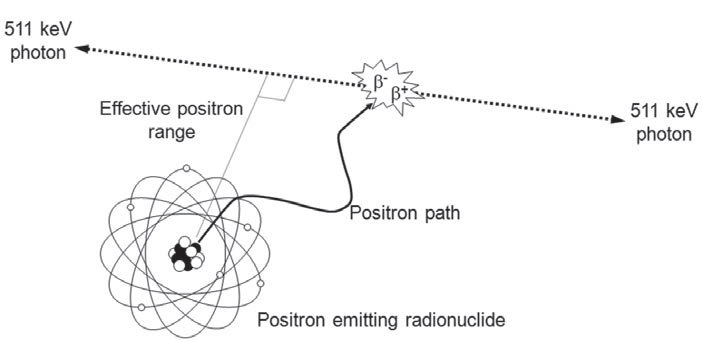
\includegraphics[width=0.8\linewidth]{./ImageFiles/annihilation}
	\caption{Processo di annichilazione \textit{positrone-elettrone} con generazione di due raggi gamma. Immagine tratta da Bailey D. et al\cite{Bailey2014}.}
	\label{fig:annihilation}
\end{figure}
